\documentclass{reportx}

\NewDocumentCommand\optmodule{sO{}mmm}{%
    \IfBooleanTF{#1}{%
        \begin{equation*}
            \ifthenelse{\equal{#2}{}}{}{(#2)\quad}
            \begin{aligned}
                \begin{cases}
                    #3 \quad & #4 \\
                    \mathrm{s.t.} \quad #5
                \end{cases}
            \end{aligned}
        \end{equation*}
    }{%
        \begin{equation}
            \ifthenelse{\equal{#2}{}}{}{(#2)\quad}
            \begin{aligned}
                \begin{cases}
                    #3 \quad & #4 \\
                    \mathrm{s.t.} \quad #5
                \end{cases}
            \end{aligned}
        \end{equation}
    }%
}

\begin{document}
    \section{实验内容}

本实验将进行如下工作:

第一, 介绍各种典型的优化方法.
将系统地梳理优化算法的基本分类与原理, 涵盖从无需梯度信息的无导数优化方法到依赖梯度信息的有导数优化方法.
在一阶优化器部分, 将重点讲解基于梯度信息的优化策略, 包括最基本的梯度下降法、适用于非光滑目标函数的次梯度下降法, 以及加速收敛的共轭方向法、共轭梯度法和采用迭代更新Hessian矩阵近似的变尺度法(如BFGS法).
二阶优化器则引入目标函数的Hessian矩阵以提升收敛速度, 典型方法包括Newton法与其改进形式阻尼Newton法, 后者通过调整Hessian矩阵提升算法稳定性.
此外, 还将介绍交替方向乘子法(ADMM)这种适用于分布式和约束优化问题的有效算法, 以及Krylov子空间方法等在高维大规模问题中应用广泛的迭代式优化策略.

第二, 实现上述优化方法.
利用Python编程语言实现所介绍的各类优化算法.
为了确保每种方法具有通用性和可扩展性, 将使用PyTorch框架对各种优化器进行实现, 继承Optimizer接口, 便于后续在不同类型的目标函数上进行测试和比较.

第三, 测试上述优化方法.
使用一个典型的测试函数对各优化器进行性能评估——Rosenbrock函数.
实验将对每种优化器在在相同初始点下的收敛过程进行可视化分析, 并对优化器性能进行比较.

    \section{优化方法介绍}

\subsection{随机搜索法}

随机搜索法(Random Search Method)是一种无导数优化方法,其基本思想是在定义域内随机生成若干点,并选择函数值最小的作为当前最优解。
设优化问题为
\begin{equation*}
    \min_{\bm{x}\in\mathbb{R}^n} ~ f(\bm{x}) \text{。}
\end{equation*}
在第$k$次迭代中,随机生成点$\bm{x}_k'\in U(\bm{x}_k)$,其中$U(\bm{x}_k)$为$\bm{x}_k$的某一邻域。

则有迭代公式
\begin{equation*}
    \bm{x}_{k+1}=\bm{x}_k'
    \begin{cases}
        \bm{x}_k'\text{,} &f(\bm{x}_k')<f(\bm{x}_k) \text{,} \\
        \bm{x}_k\text{,} &f(\bm{x}_k')\geq f(\bm{x}_k) \text{。}
    \end{cases}
\end{equation*}
该方法通过不断试探更新寻找函数值更小的位置,而无需任何梯度信息。

\subsection{梯度下降法}

梯度下降法(Gradient Descent Method)利用目标函数的梯度信息,以梯度的负方向作为下降方向,即
\begin{equation*}
    \bm{x}_{k+1}=\bm{x}_k-\alpha_k\nabla f(\bm{x}_k) \text{,}
\end{equation*}
其中$\alpha_k>0$为学习率,$\nabla f(\bm{x}_k)$为目标函数在点$\bm{x}_k$处的梯度。

\subsection{次梯度下降法}

次梯度下降法(Subgradient Descent Method)用于优化非光滑凸函数。
若$f$在点$\bm{x}_k$处不可导,但存在次梯度$\bm{g}_k\in\partial f(\bm{x}_k)$, 则有
\begin{equation*}
    \bm{x}_{k+1}=\bm{x}_k-\alpha_k\bm{g}_k \text{,}
\end{equation*}
其中$\alpha_k>0$为学习率,$\partial f(\bm{x}_k)$为目标函数在点$\bm{x}_k$处的次梯度集合。

\subsection{共轭方向法}

共轭方向法(Conjugate Direction Method)用于二次函数
\begin{equation*}
    f(\bm{x})=\frac{1}{2}\bm{x}^\mathrm{T}\bm{Ax}-\bm{b}^\mathrm{T}\bm{x} \text{,}
\end{equation*}
其中矩阵$\bm{A}$对称正定。

共轭方向法需要构造一组关于矩阵$\bm{A}$的共轭方向$\{\bm{d}_i\}_{i=1}^n$,使得
\begin{equation*}
    \bm{d}_i\bm{A}\bm{d}_j=0 \text{,} i\ne j \text{,}
\end{equation*}
沿着这些方向进行线性搜索,即
\begin{equation*}
    \bm{x}_{k+1}=\bm{x}_k-\alpha_k\bm{d}_k \text{,}
\end{equation*}
其中$\alpha_k>0$为学习率,可通过一维搜索得到。

\subsection{共轭梯度法}

共轭梯度法(Conjugate Gradient Method)是一种特殊的共轭方向法,使用当前梯度和上一次方向构造共轭方向,避免计算$\bm{A}$。
对于二次函数,其迭代格式为:
\begin{align*}
    &\bm{x}_{k+1}=\bm{x}_k-\alpha_k\bm{d}_k \text{,} \\
    &\alpha_k=\frac{\bm{r}_k^\mathrm{T}\bm{r}_k}{\bm{d}_k^\mathrm{T}\bm{Ad}_k} \text{,} \\
    &\bm{d}_k=\bm{r}_k+\beta_{k-1}\bm{d}_{k-1} \text{,} \beta_{k-1}=\frac{\bm{r}_k^\mathrm{T}\bm{r}_k}{\bm{r}_{k-1}^\mathrm{T}\bm{r}_{k-1}} \text{,} \\
    &\bm{r}_k=\bm{b}-\bm{Ax}_k \text{,} \bm{r}_0=-\nabla f(\bm{x}_0) \text{。}
\end{align*}

    \section{实验设置及结果}

为了使优化器的通用性和可扩展性,实验基于PyTorch的Optimizer类进行优化器实现,并分别实现了随机搜索优化器,梯度下降优化器,次梯度下降优化器,共轭方向优化器,共轭梯度优化器,变尺度法优化器(BFGS),随机梯度下降优化器,Newton优化器,阻尼Newton优化器,ADMM优化器和Krylov子空间优化器,并使用Rosenbrock Banana函数作为优化器测试函数,即
\begin{equation*}
    f(x_1, x_2)=(a-x_1)^2-b(x_2-x_1^2)^2 \text{,}
\end{equation*}
其中$a=1$,$b=-100$。
实验结果如\cref{table:result}所示,各优化器的最优值收敛曲线和最优点收敛路径如\cref{figure:random search}至\cref{figure:krylov}所示。

\begin{table}[ht]
    \centering
    \caption{实验结果}
    \label{table:result}
    \begin{tabular}{cccc}
        \toprule
        \textbf{优化器} & \textbf{最优点} & \textbf{最优值} & \textbf{迭代轮次} \\
        \midrule
        Random Search & $(1.00, 1.00)$ & 0.00 & 1326 \\
        Gradient Descent & $(0.99, 1.00)$ & 0.00 & 10808 \\
        Subgradient Descent & $(0.99, 1.00)$ & 0.00 & 10808 \\
        Conjugate Direction & $(1.00, 1.00)$ & 0.00 & 23366 \\
        Conjugate Gradient & $(1.00, 1.00)$ & 0.00 & 500 \\
        BFGS & $(1.00, 1.00)$ & 0.00 & 21983 \\
        SGD & $(1.00, 1.00)$ & 0.00 & 6350 \\
        Newton & $(1.00, 1.00)$ & 0.00 & 7 \\
        Damped Newton & $(1.00, 1.00)$ & 0.00 & 2970 \\
        ADMM & $(1.00, 1.00)$ & 0.00 & 22184 \\
        Krylov & $(1.00, 1.00)$ & 0.00 & 6385 \\
        \bottomrule
    \end{tabular}
\end{table}

\begin{figure}[!ht]
    \centering
    \begin{subfigure}{0.4\textwidth}
        \centering
        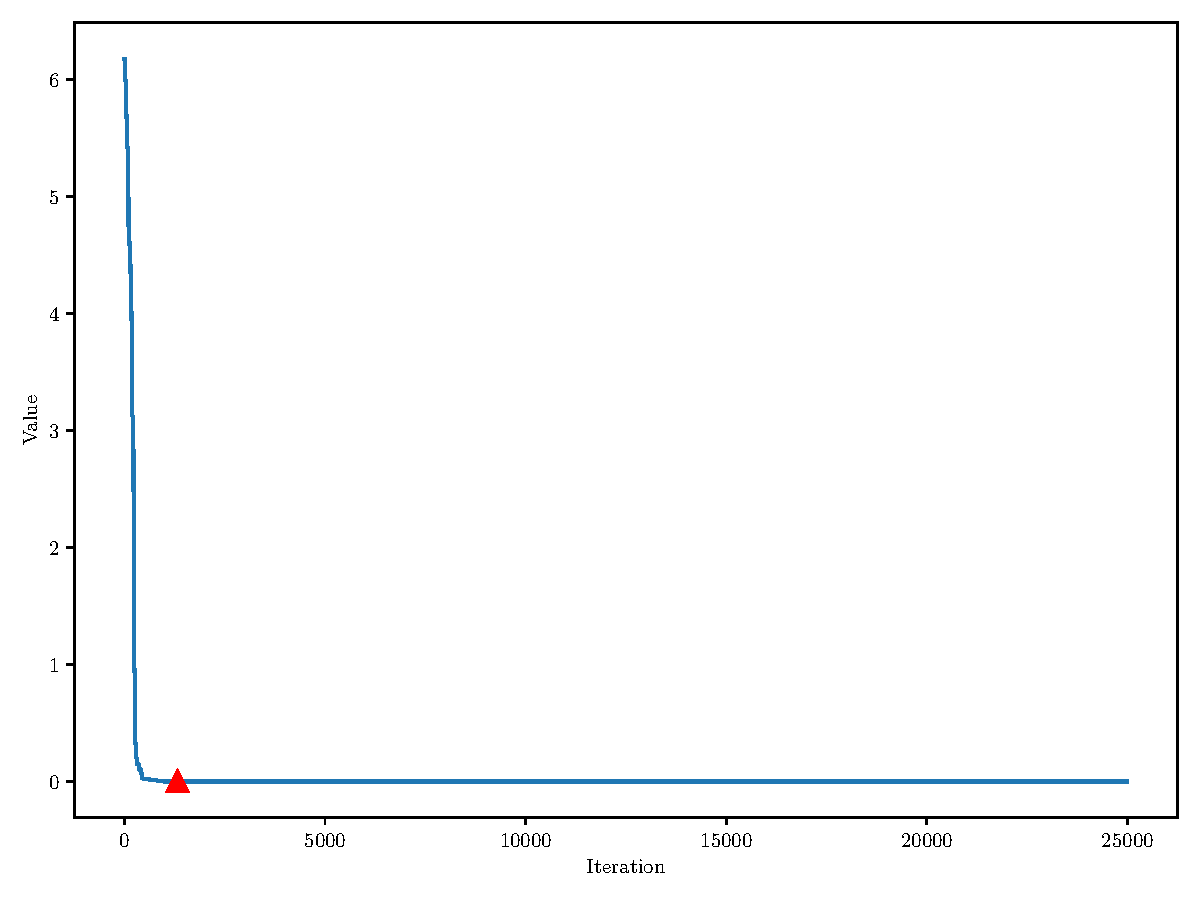
\includegraphics[width=\textwidth]{figures/Random Search_loss.pdf}
        \caption{最优值收敛曲线}
    \end{subfigure}
    \begin{subfigure}{0.4\textwidth}
        \centering
        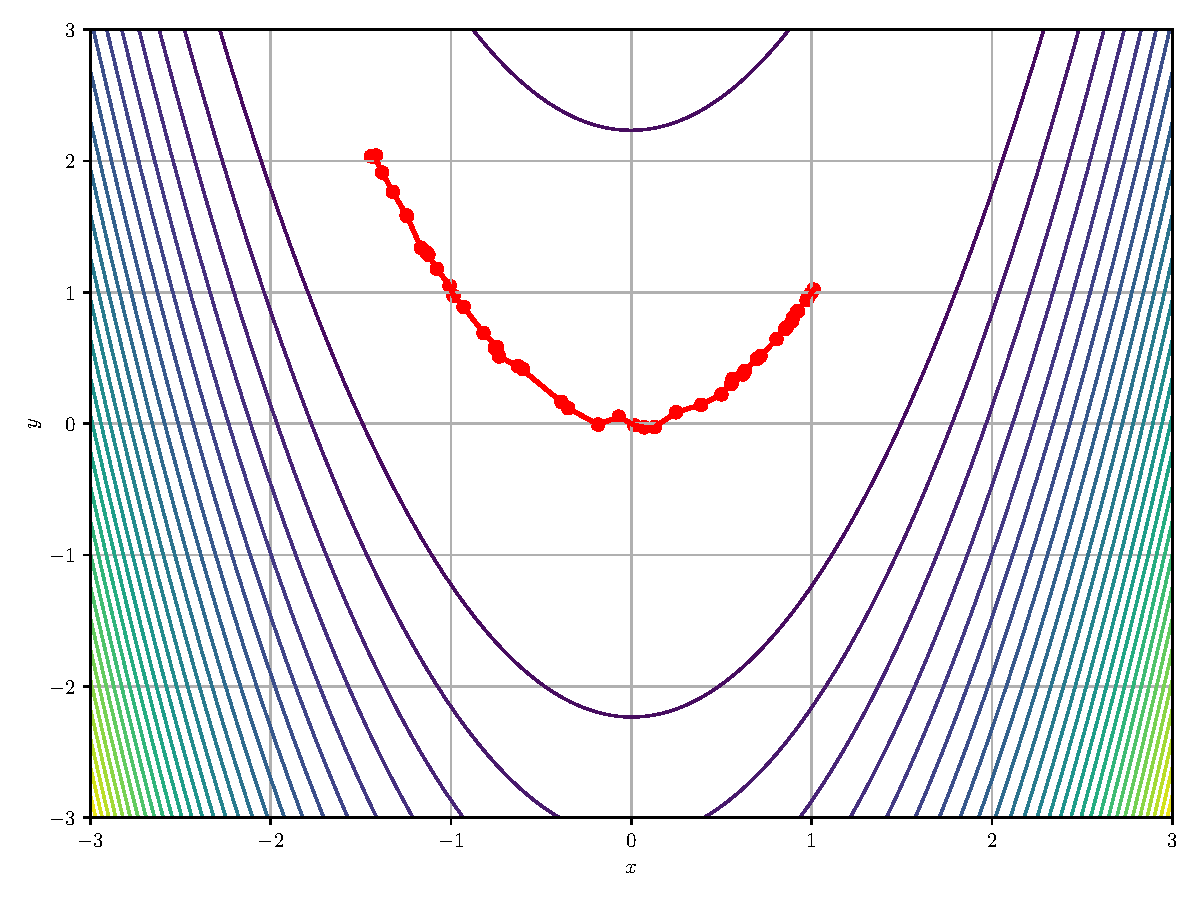
\includegraphics[width=\textwidth]{figures/Random Search_points.pdf}
        \caption{最优点收敛路径}
    \end{subfigure}
    \caption{Random Search的最优值收敛曲线与最优点收敛路径}
    \label{figure:random search}
\end{figure}
\begin{figure}[!ht]
    \centering
    \begin{subfigure}{0.4\textwidth}
        \centering
        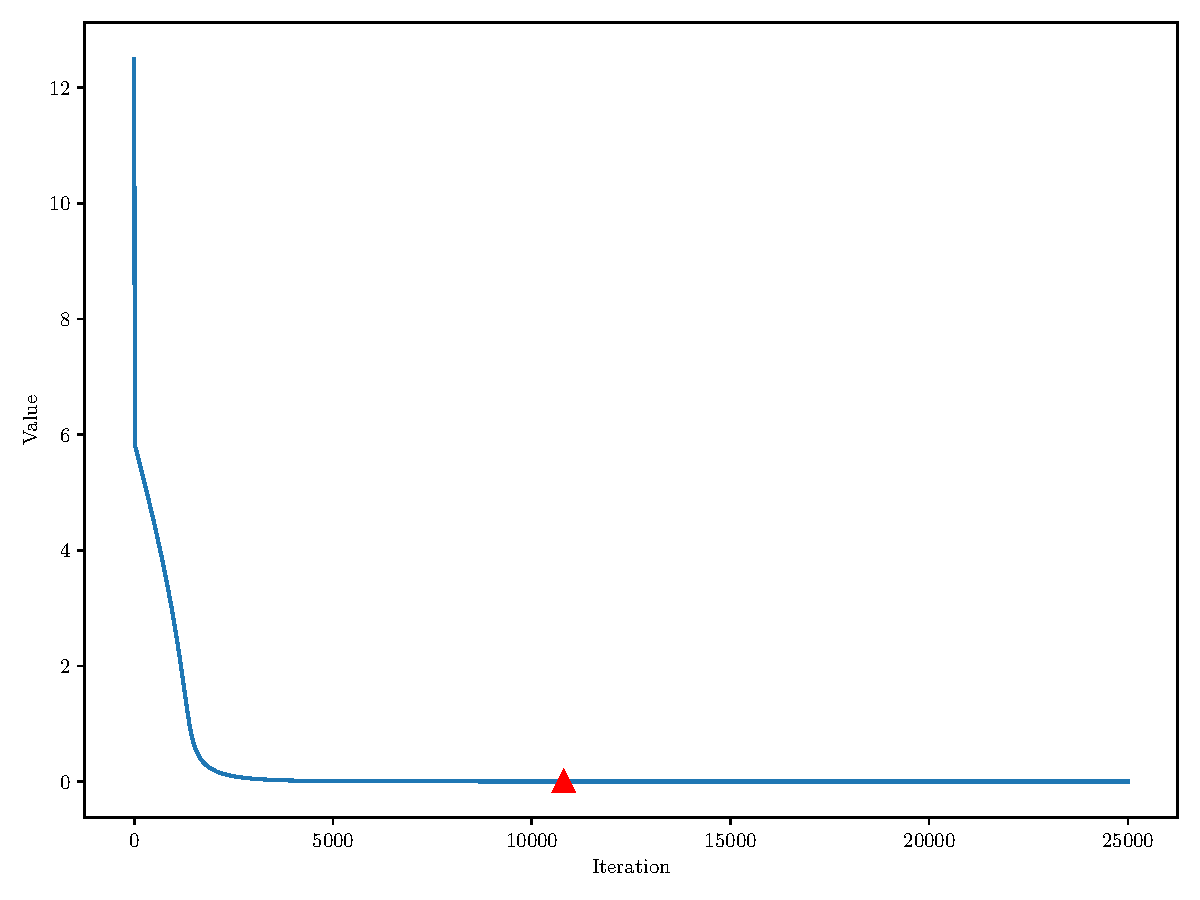
\includegraphics[width=\textwidth]{figures/Gradient Descent_loss.pdf}
        \caption{最优值收敛曲线}
    \end{subfigure}
    \begin{subfigure}{0.4\textwidth}
        \centering
        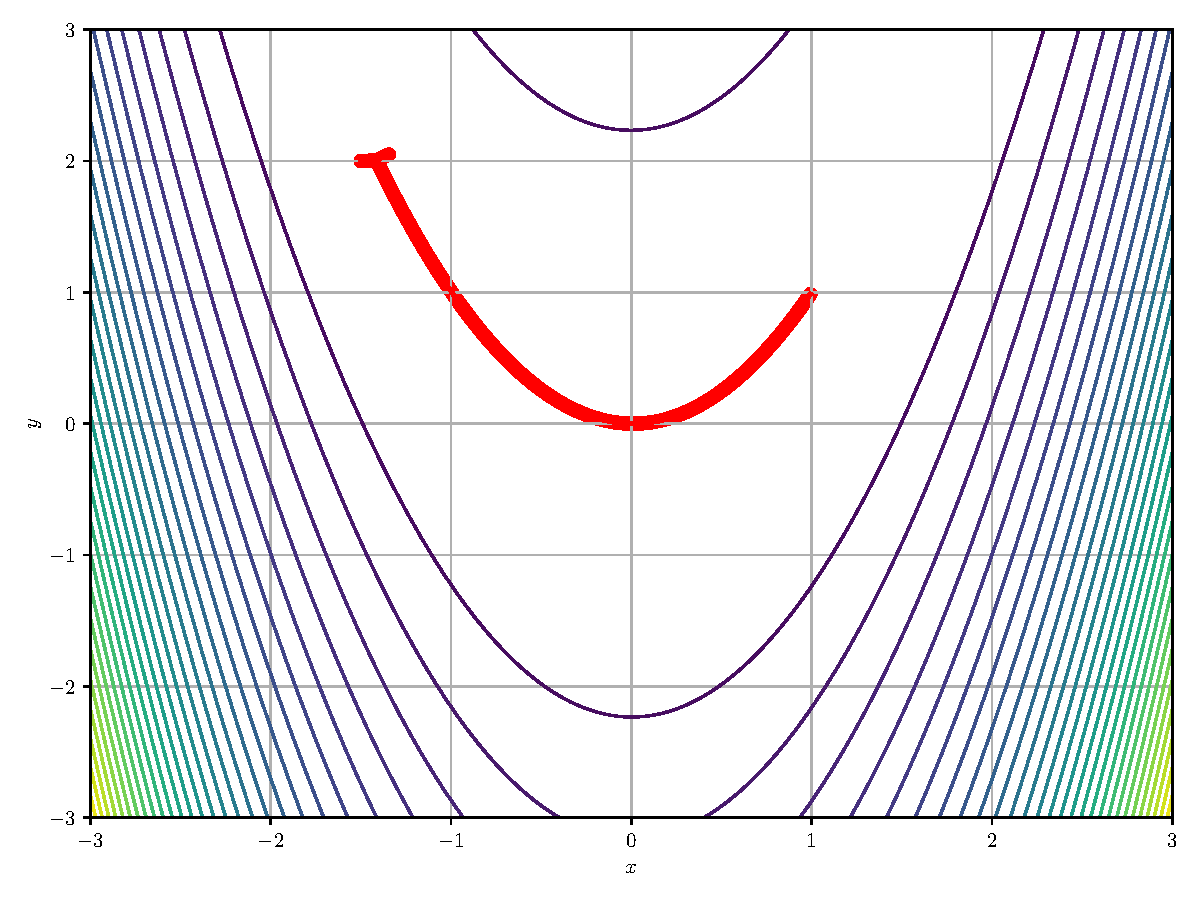
\includegraphics[width=\textwidth]{figures/Gradient Descent_points.pdf}
        \caption{最优点收敛路径}
    \end{subfigure}
    \caption{Gradient Descent的最优值收敛曲线与最优点收敛路径}
\end{figure}
\begin{figure}[!ht]
    \centering
    \begin{subfigure}{0.4\textwidth}
        \centering
        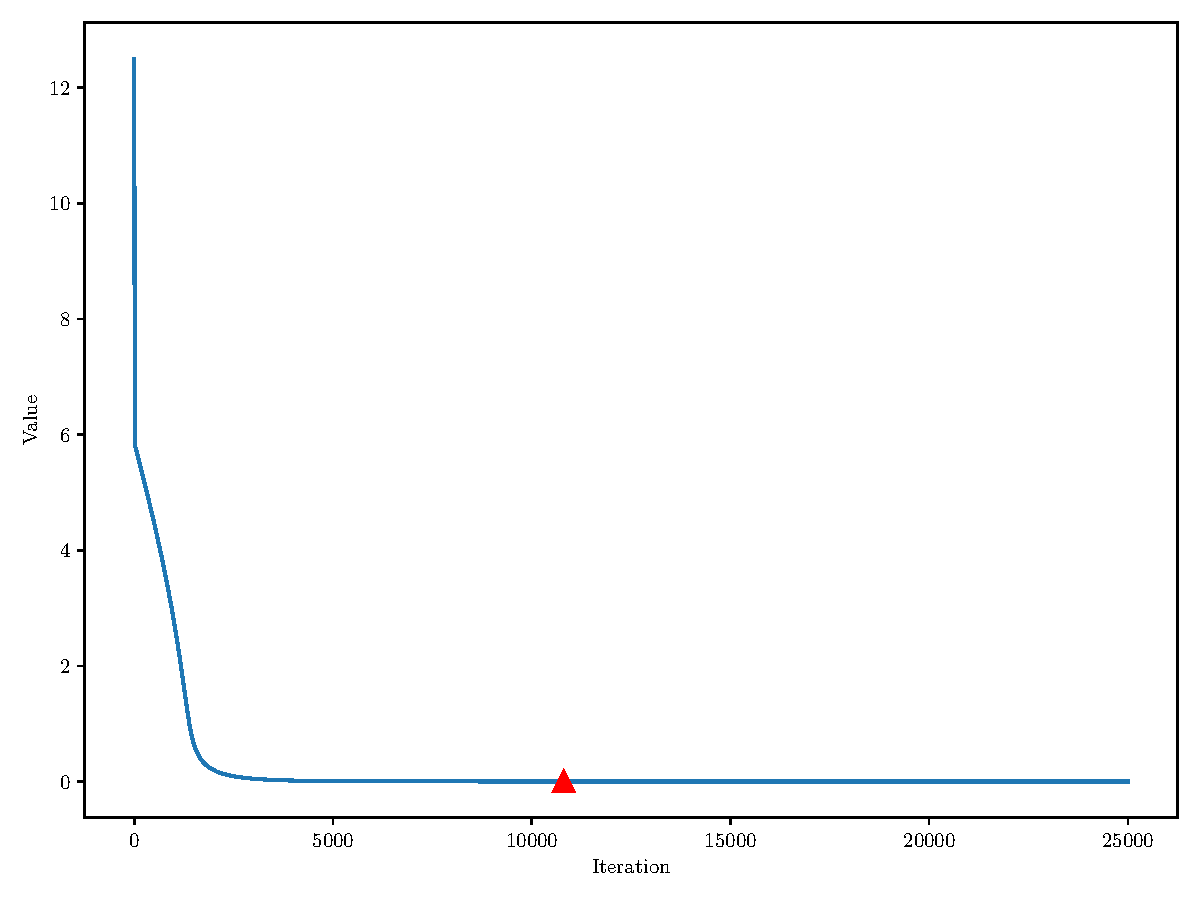
\includegraphics[width=\textwidth]{figures/Subgradient Descent_loss.pdf}
        \caption{最优值收敛曲线}
    \end{subfigure}
    \begin{subfigure}{0.4\textwidth}
        \centering
        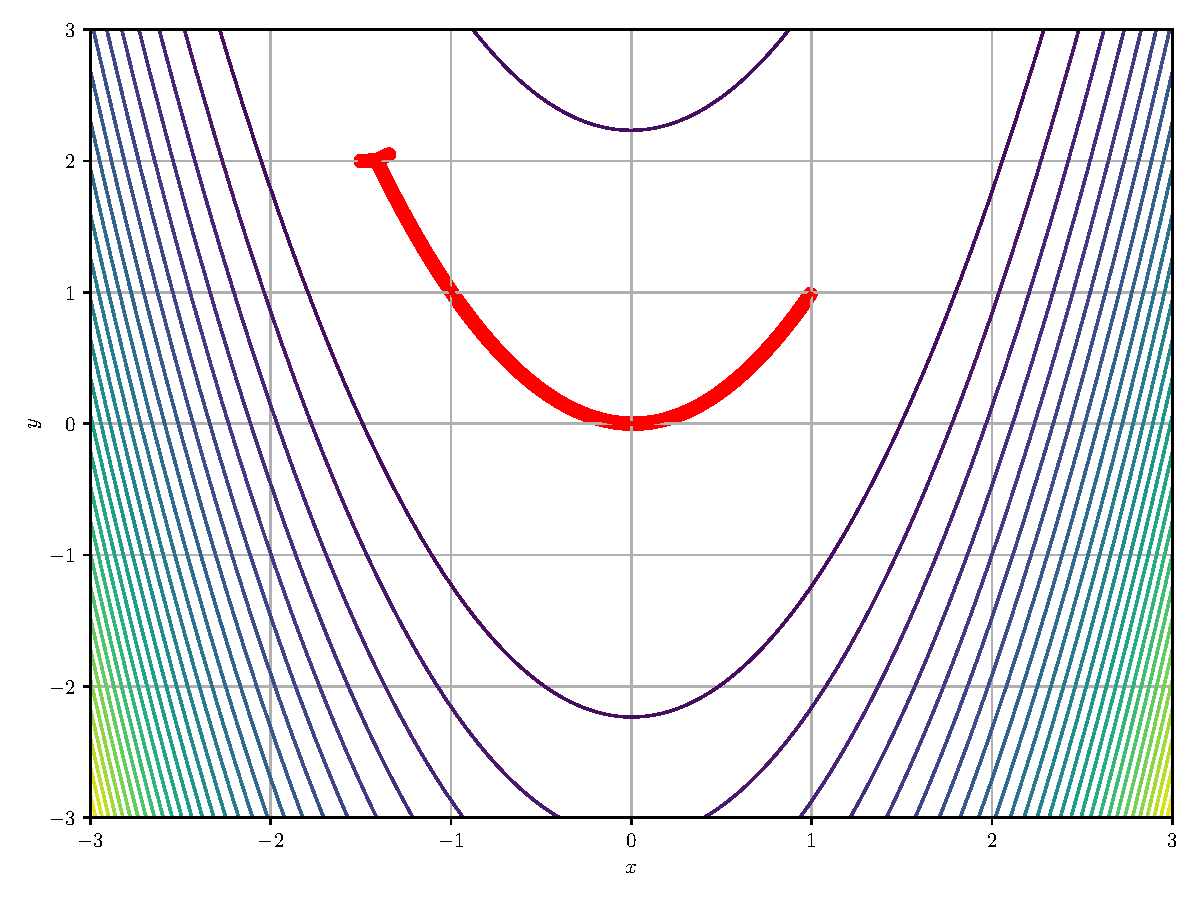
\includegraphics[width=\textwidth]{figures/Subgradient Descent_points.pdf}
        \caption{最优点收敛路径}
    \end{subfigure}
    \caption{Subgradient Descent的最优值收敛曲线与最优点收敛路径}
\end{figure}
\begin{figure}[!ht]
    \centering
    \begin{subfigure}{0.4\textwidth}
        \centering
        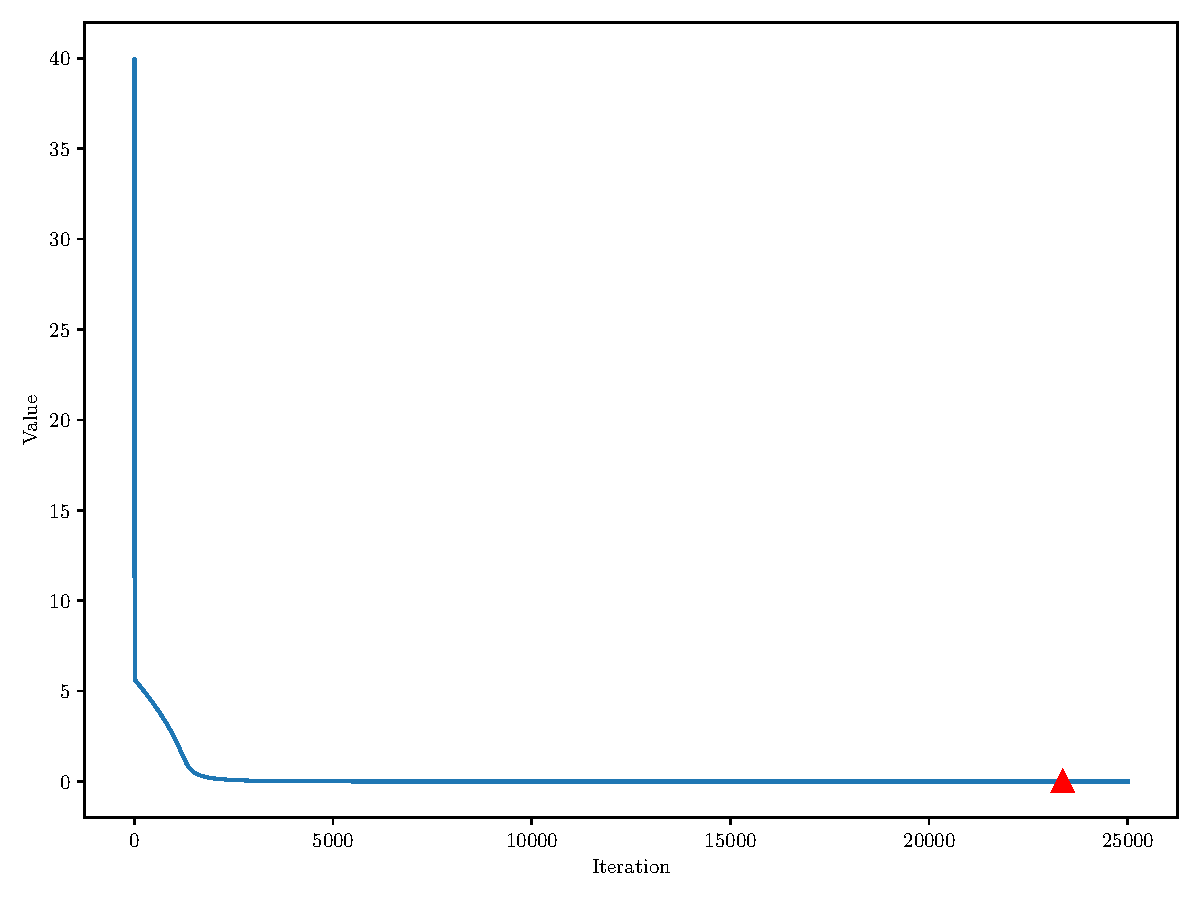
\includegraphics[width=\textwidth]{figures/Conjugate Direction_loss.pdf}
        \caption{最优值收敛曲线}
    \end{subfigure}
    \begin{subfigure}{0.4\textwidth}
        \centering
        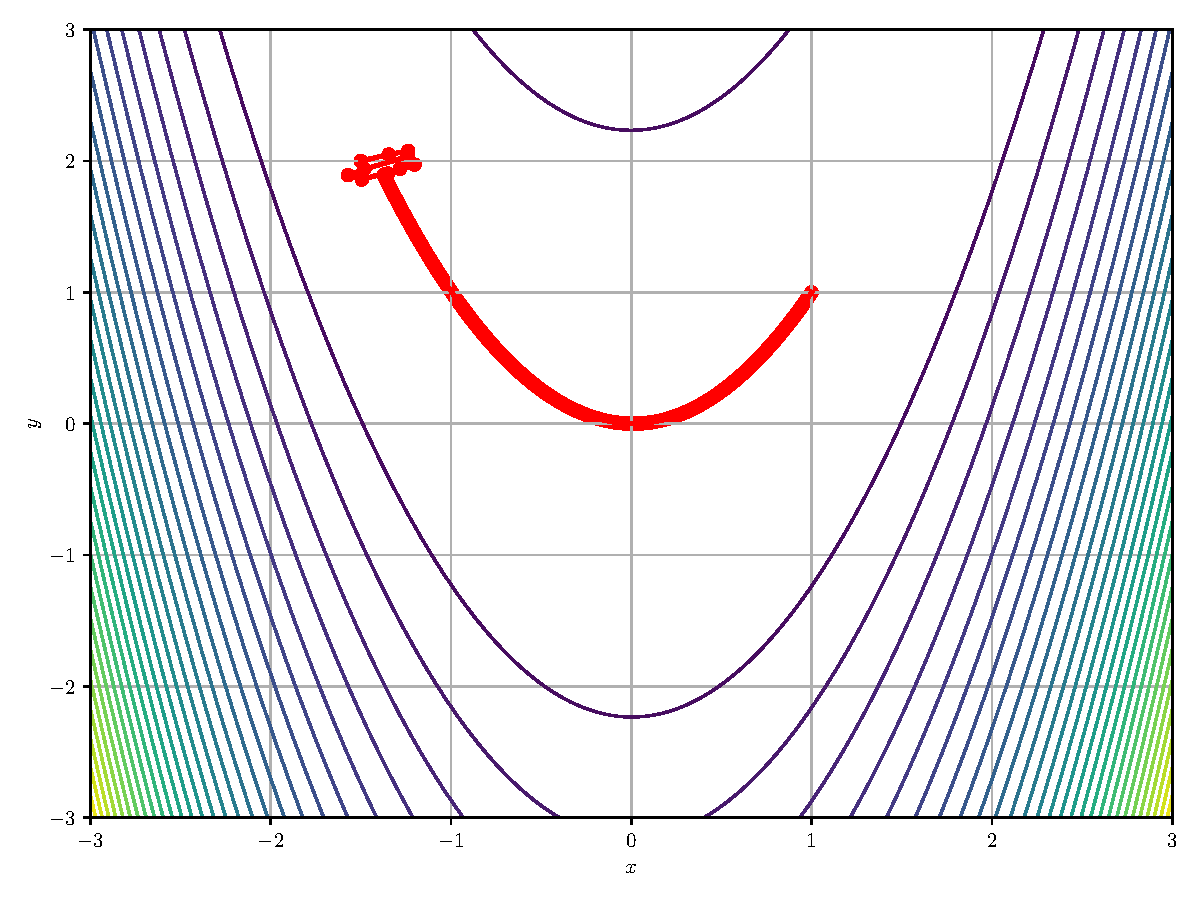
\includegraphics[width=\textwidth]{figures/Conjugate Direction_points.pdf}
        \caption{最优点收敛路径}
    \end{subfigure}
    \caption{Conjugate Direction的最优值收敛曲线与最优点收敛路径}
\end{figure}
\begin{figure}[!ht]
    \centering
    \begin{subfigure}{0.4\textwidth}
        \centering
        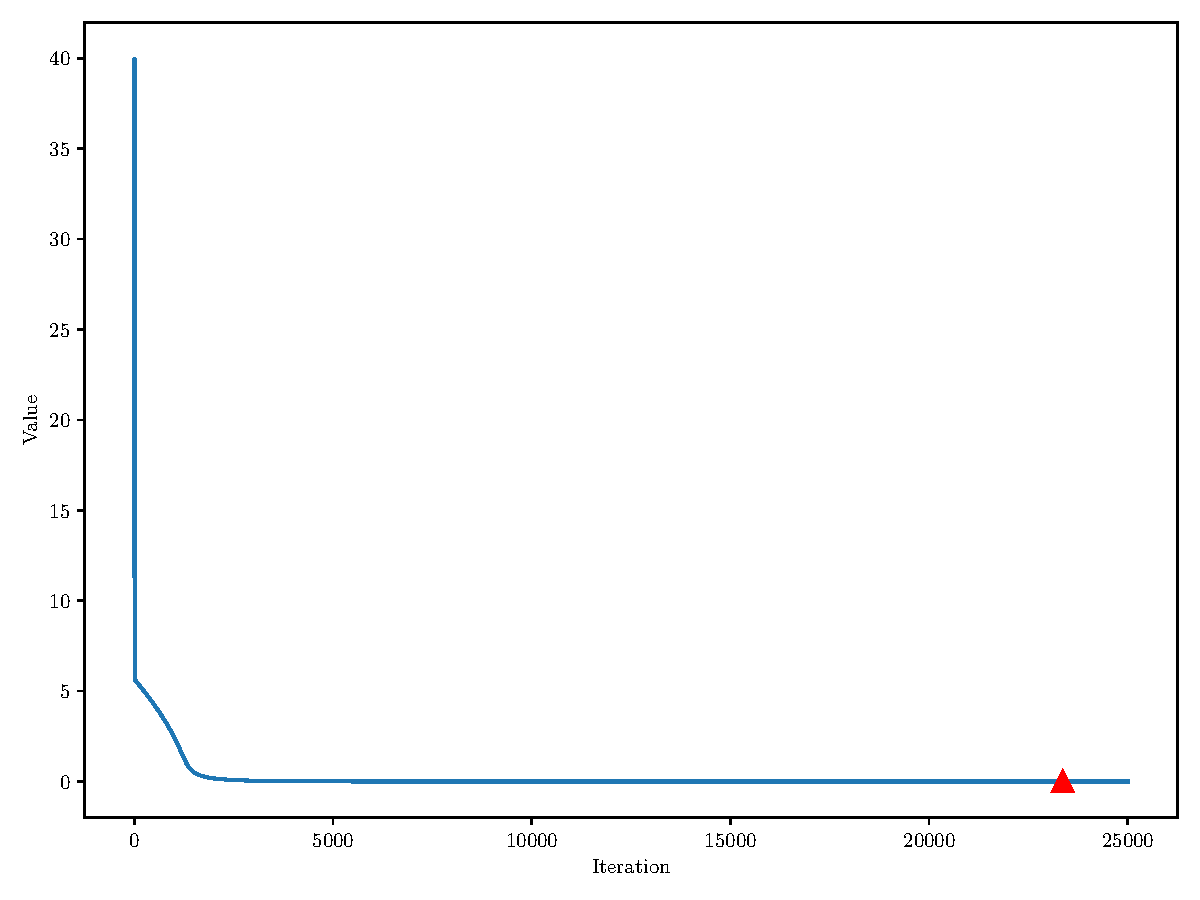
\includegraphics[width=\textwidth]{figures/Conjugate Gradient_loss.pdf}
        \caption{最优值收敛曲线}
    \end{subfigure}
    \begin{subfigure}{0.4\textwidth}
        \centering
        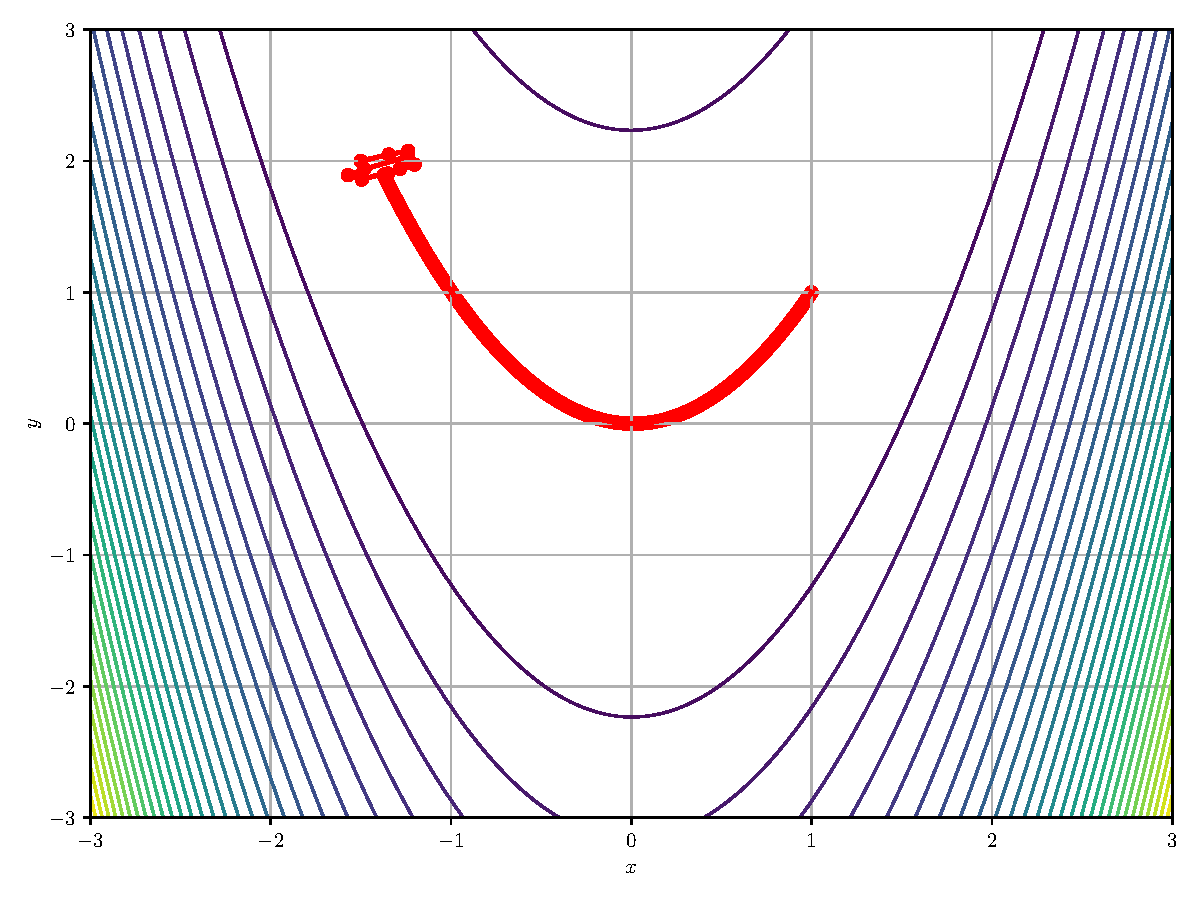
\includegraphics[width=\textwidth]{figures/Conjugate Gradient_points.pdf}
        \caption{最优点收敛路径}
    \end{subfigure}
    \caption{Conjugate Gradient的最优值收敛曲线与最优点收敛路径}
\end{figure}
\begin{figure}[!ht]
    \centering
    \begin{subfigure}{0.4\textwidth}
        \centering
        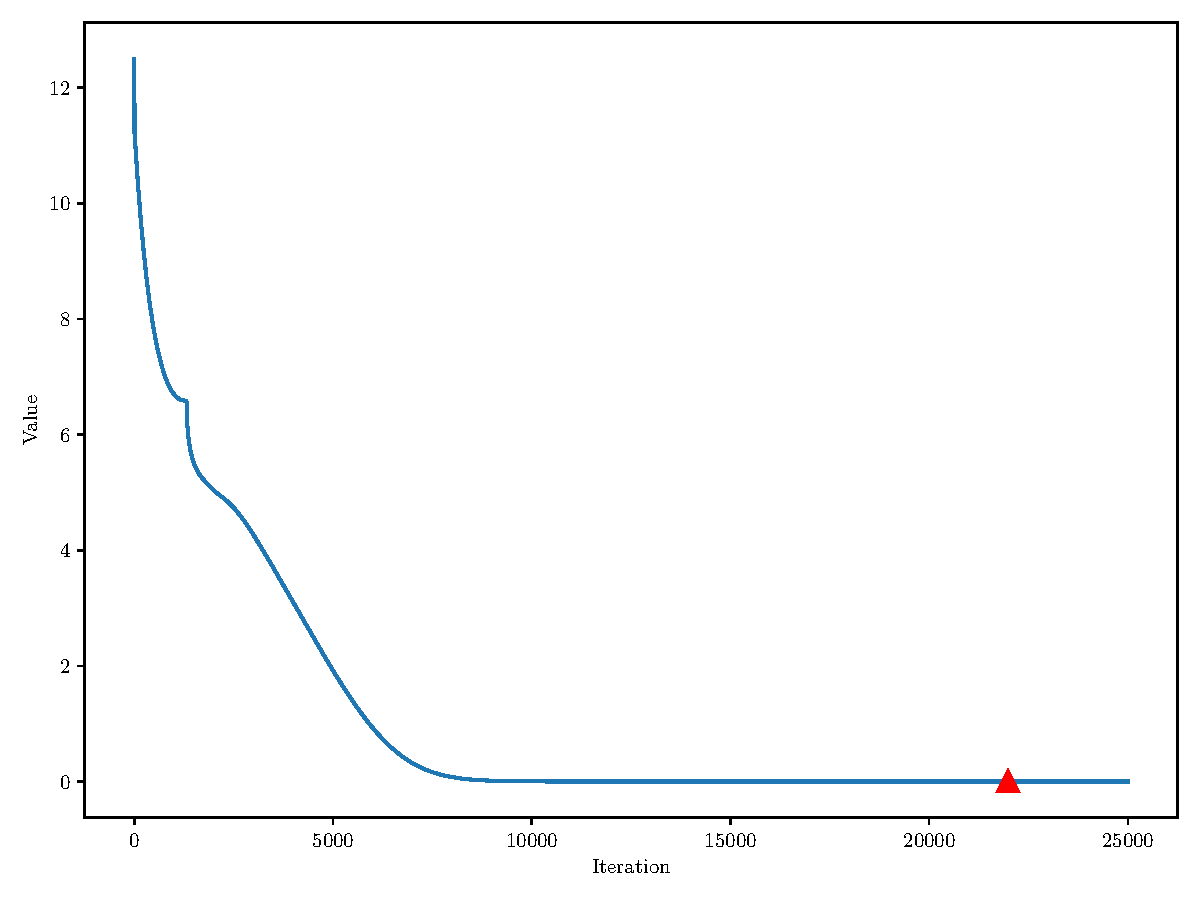
\includegraphics[width=\textwidth]{figures/BFGS_loss.pdf}
        \caption{最优值收敛曲线}
    \end{subfigure}
    \begin{subfigure}{0.4\textwidth}
        \centering
        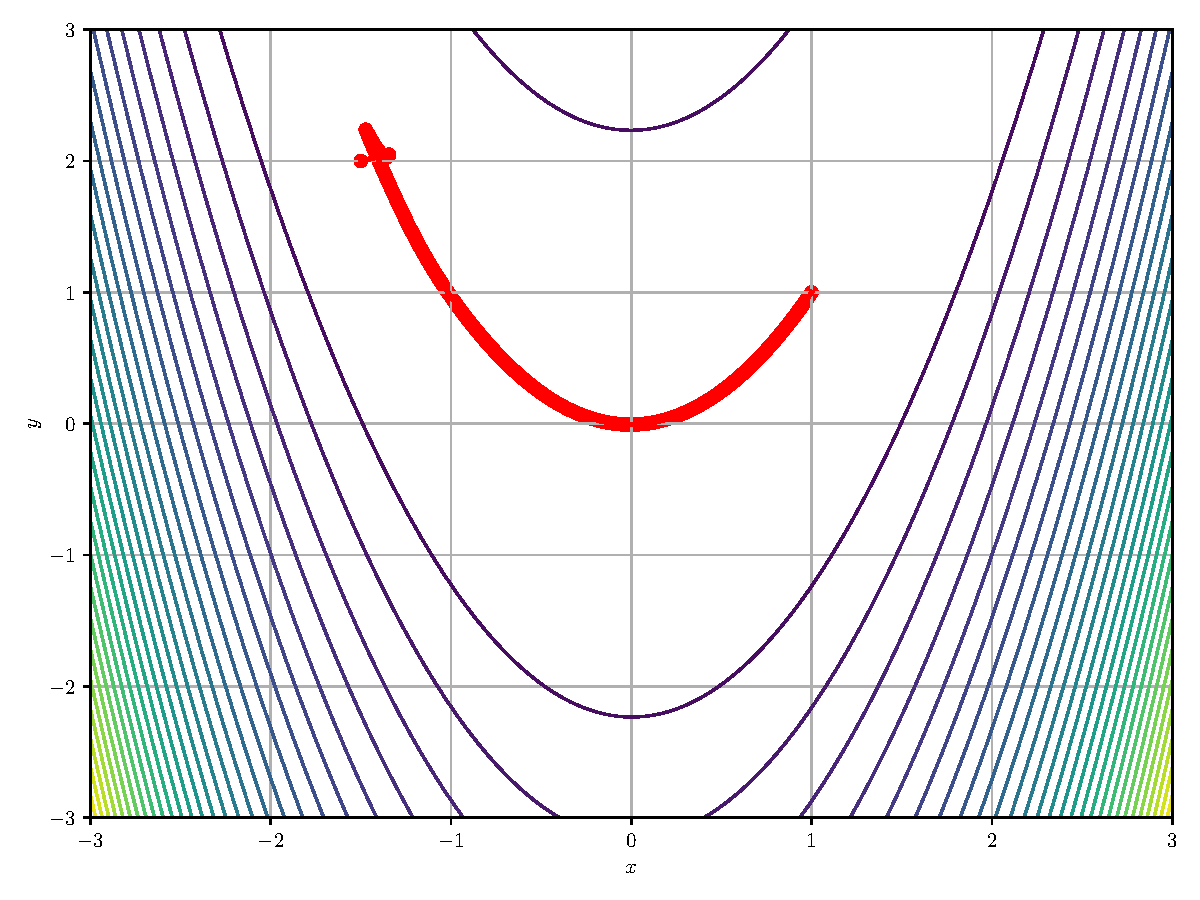
\includegraphics[width=\textwidth]{figures/BFGS_points.pdf}
        \caption{最优点收敛路径}
    \end{subfigure}
    \caption{BFGS的最优值收敛曲线与最优点收敛路径}
\end{figure}
\begin{figure}[!ht]
    \centering
    \begin{subfigure}{0.4\textwidth}
        \centering
        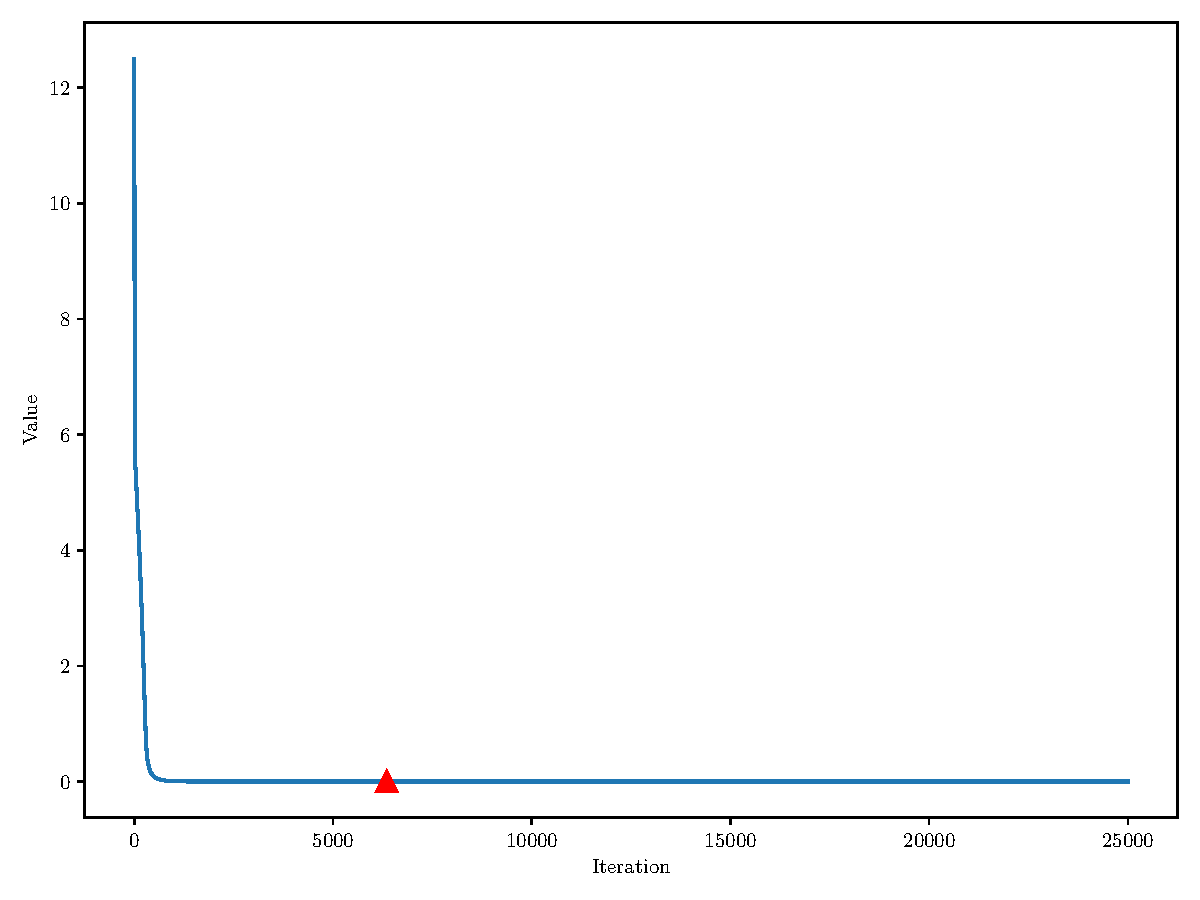
\includegraphics[width=\textwidth]{figures/SGD_loss.pdf}
        \caption{最优值收敛曲线}
    \end{subfigure}
    \begin{subfigure}{0.4\textwidth}
        \centering
        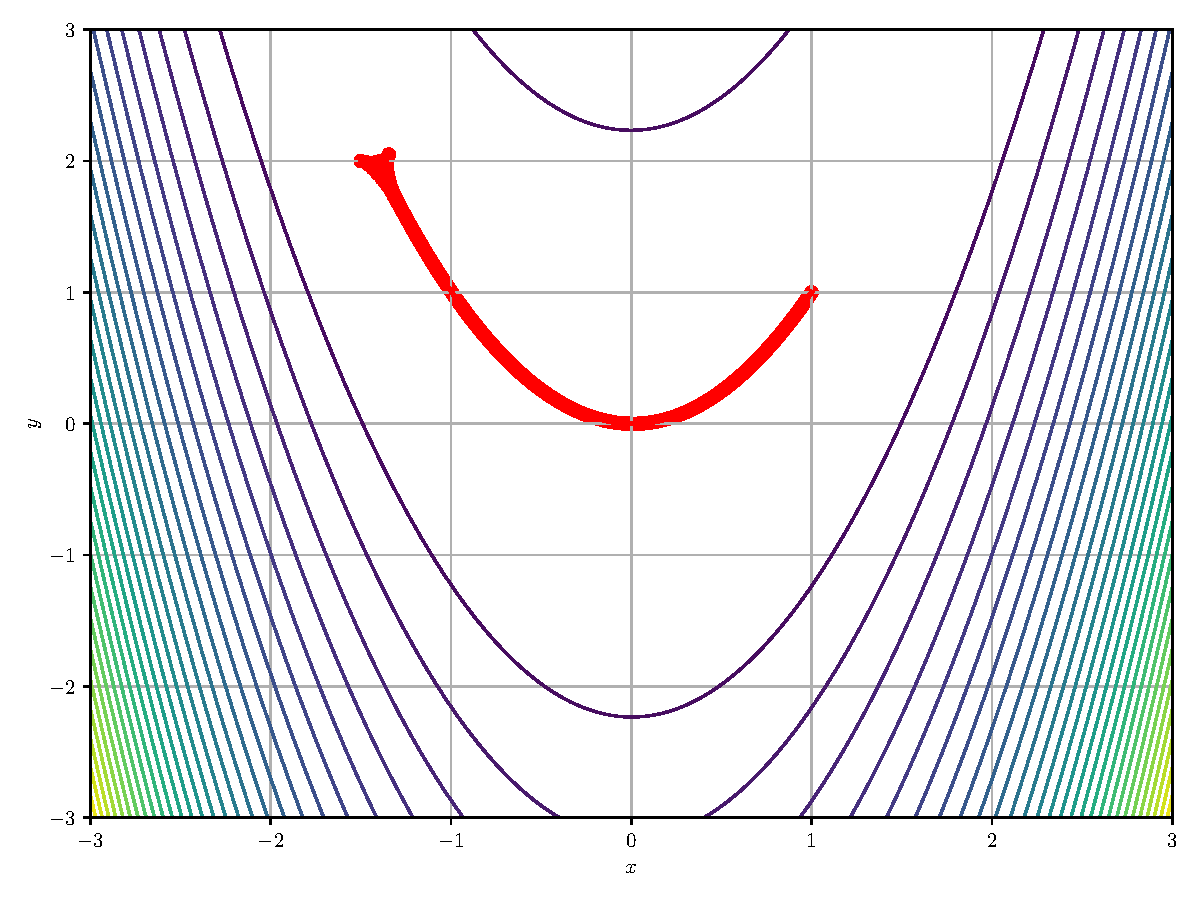
\includegraphics[width=\textwidth]{figures/SGD_points.pdf}
        \caption{最优点收敛路径}
    \end{subfigure}
    \caption{SGD的最优值收敛曲线与最优点收敛路径}
\end{figure}
\begin{figure}[!ht]
    \centering
    \begin{subfigure}{0.4\textwidth}
        \centering
        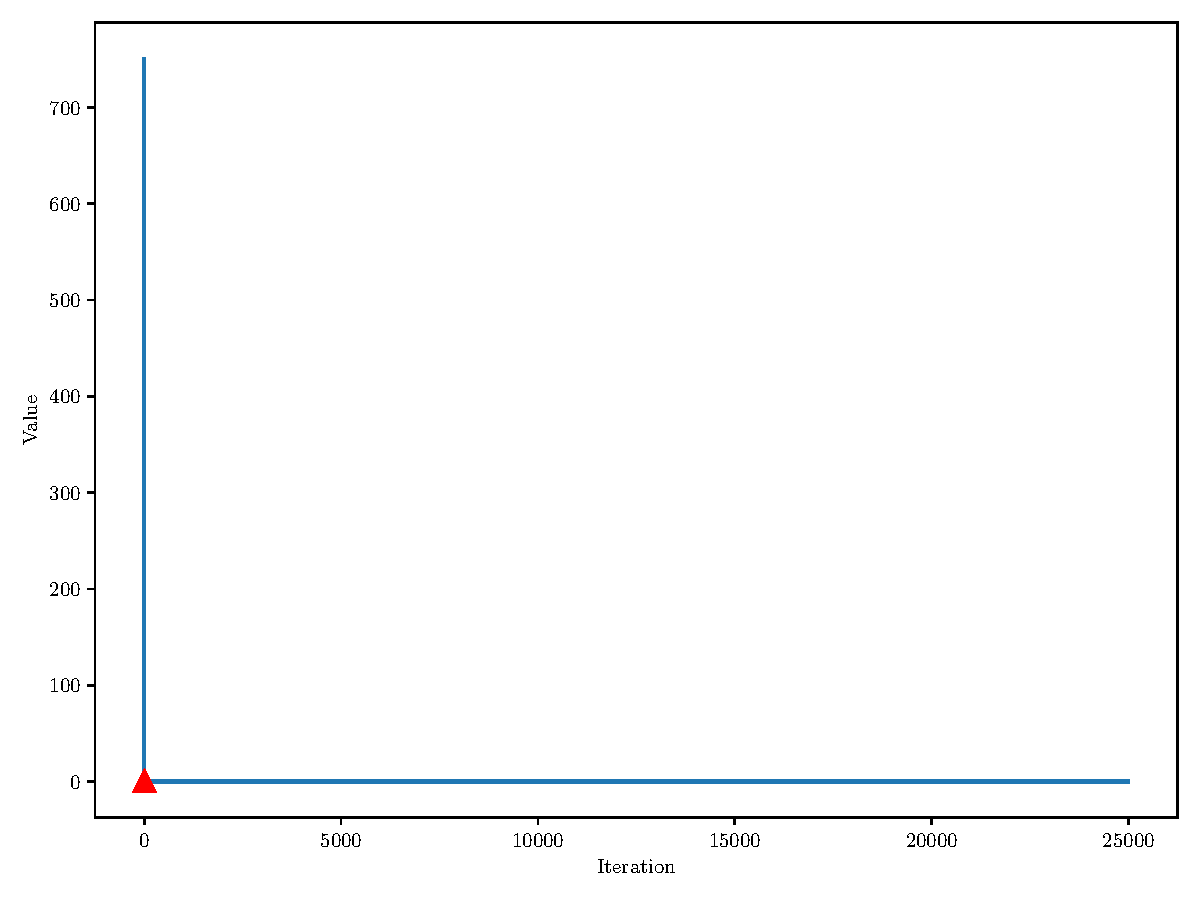
\includegraphics[width=\textwidth]{figures/Newton_loss.pdf}
        \caption{最优值收敛曲线}
    \end{subfigure}
    \begin{subfigure}{0.4\textwidth}
        \centering
        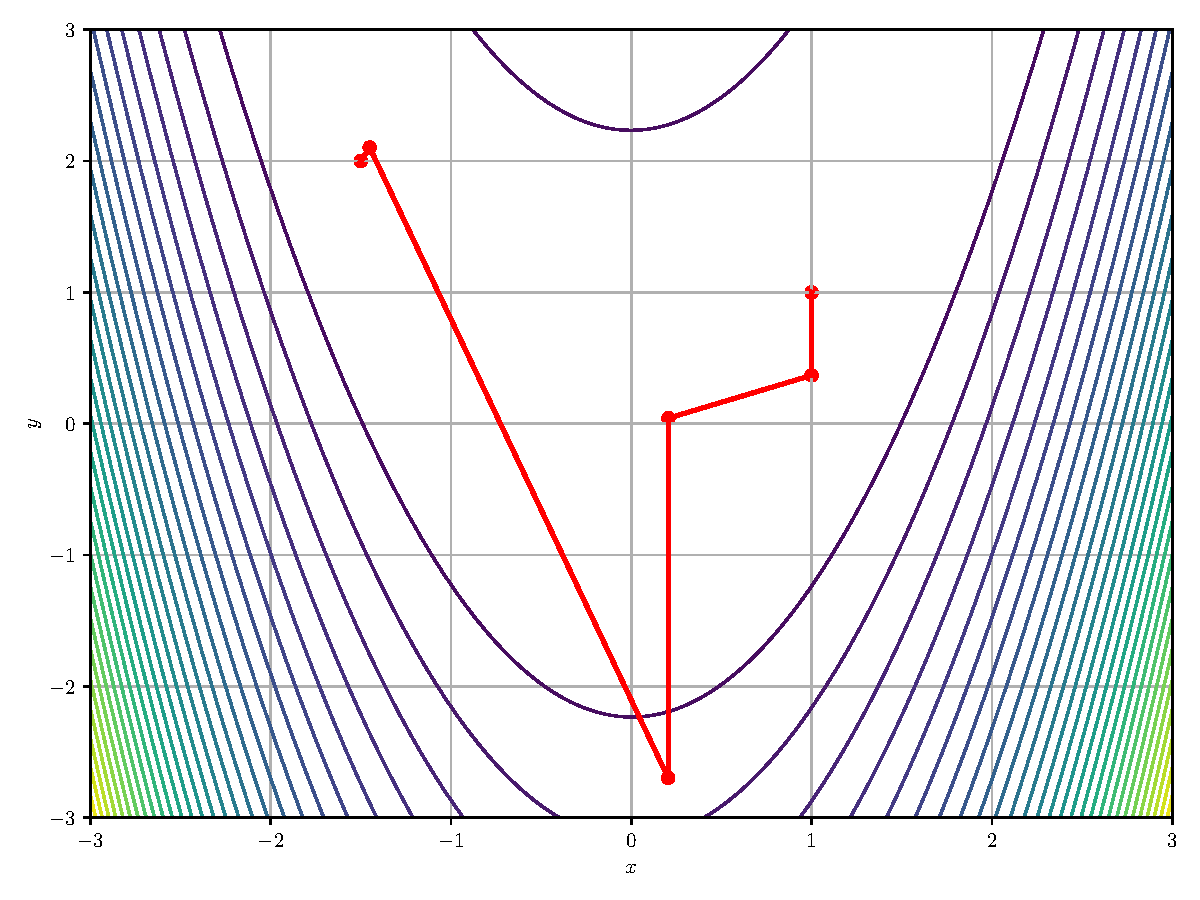
\includegraphics[width=\textwidth]{figures/Newton_points.pdf}
        \caption{最优点收敛路径}
    \end{subfigure}
    \caption{Newton的最优值收敛曲线与最优点收敛路径}
\end{figure}
\begin{figure}[!ht]
    \centering
    \begin{subfigure}{0.4\textwidth}
        \centering
        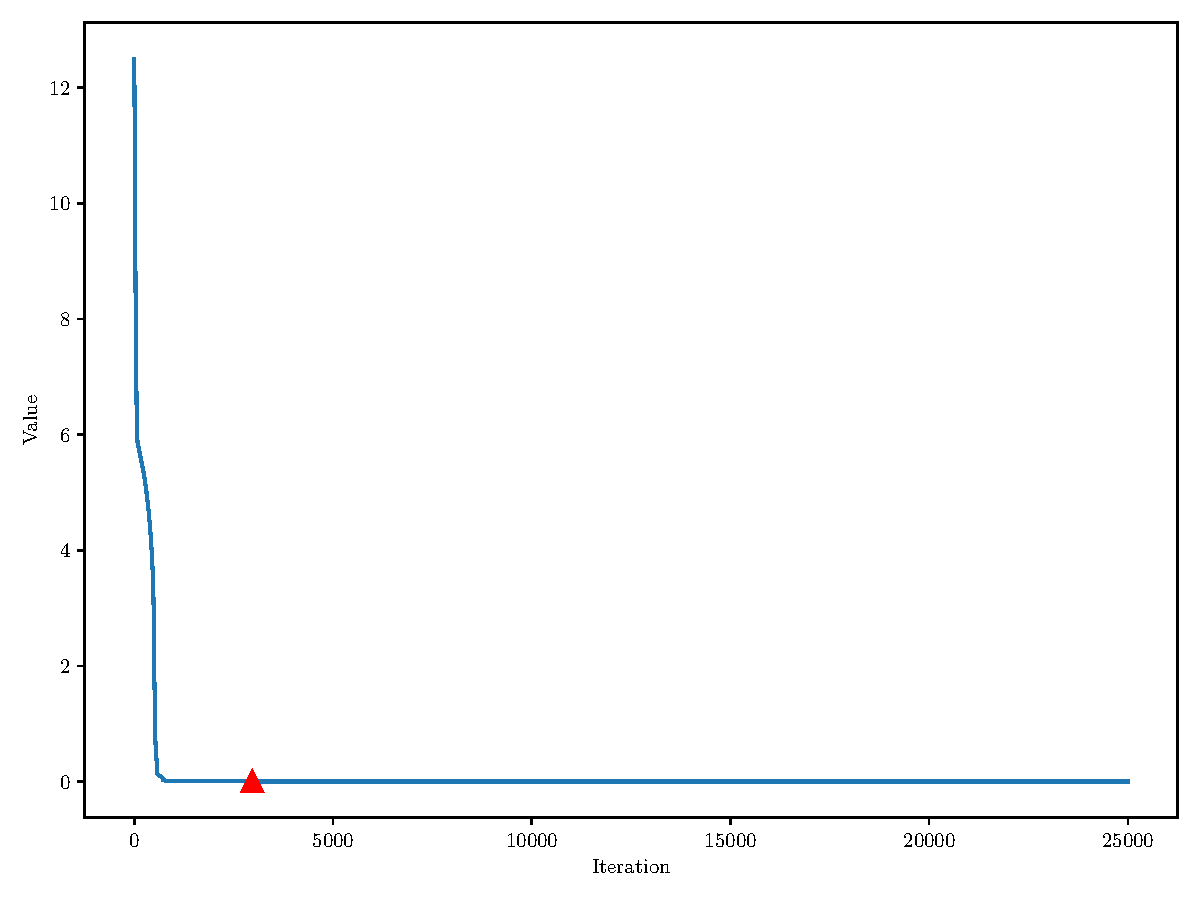
\includegraphics[width=\textwidth]{figures/Damped Newton_loss.pdf}
        \caption{最优值收敛曲线}
    \end{subfigure}
    \begin{subfigure}{0.4\textwidth}
        \centering
        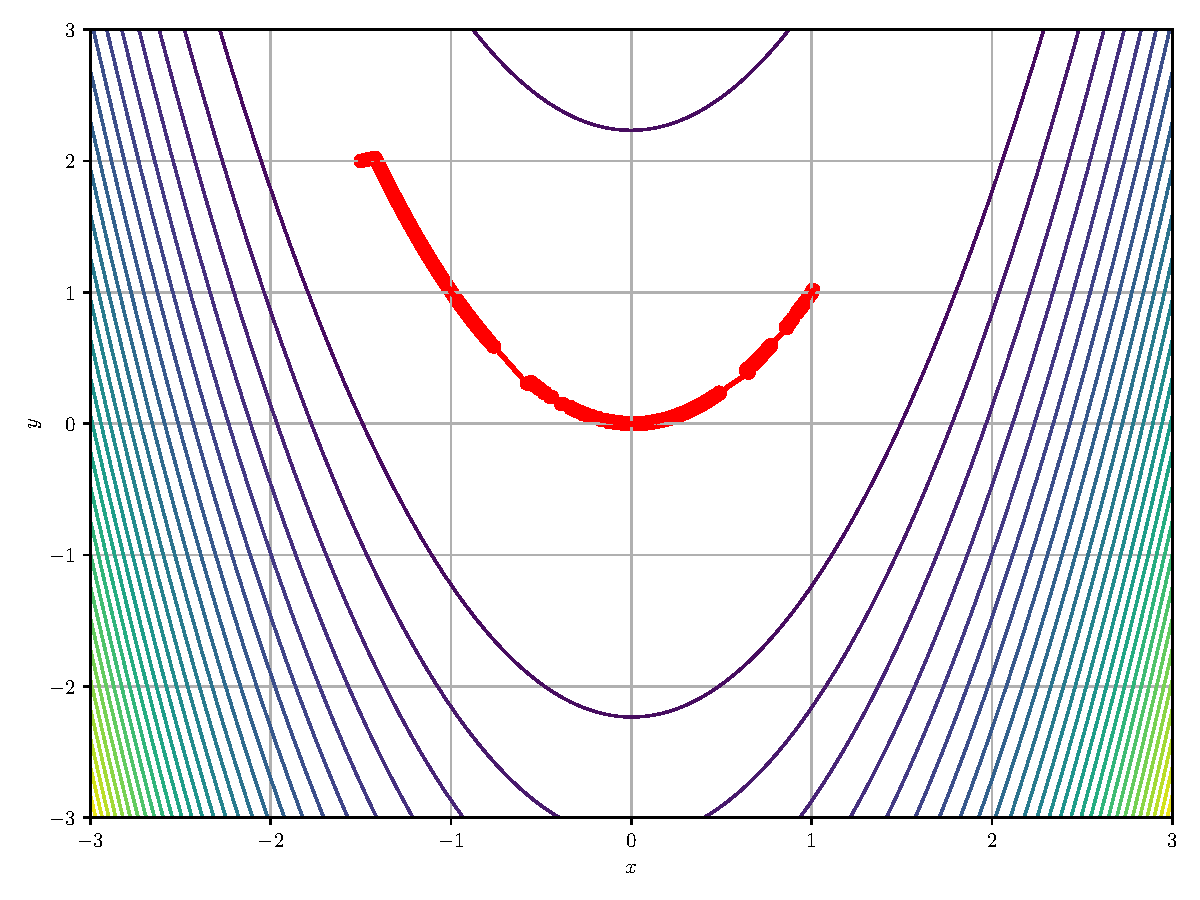
\includegraphics[width=\textwidth]{figures/Damped Newton_points.pdf}
        \caption{最优点收敛路径}
    \end{subfigure}
    \caption{Damped Newton的最优值收敛曲线与最优点收敛路径}
\end{figure}
\begin{figure}[!ht]
    \centering
    \begin{subfigure}{0.4\textwidth}
        \centering
        \includegraphics[width=\textwidth]{figures/ADMM_loss.pdf}
        \caption{最优值收敛曲线}
    \end{subfigure}
    \begin{subfigure}{0.4\textwidth}
        \centering
        \includegraphics[width=\textwidth]{figures/ADMM_points.pdf}
        \caption{最优点收敛路径}
    \end{subfigure}
    \caption{ADMM的最优值收敛曲线与最优点收敛路径}
\end{figure}
\begin{figure}[!ht]
    \centering
    \begin{subfigure}{0.4\textwidth}
        \centering
        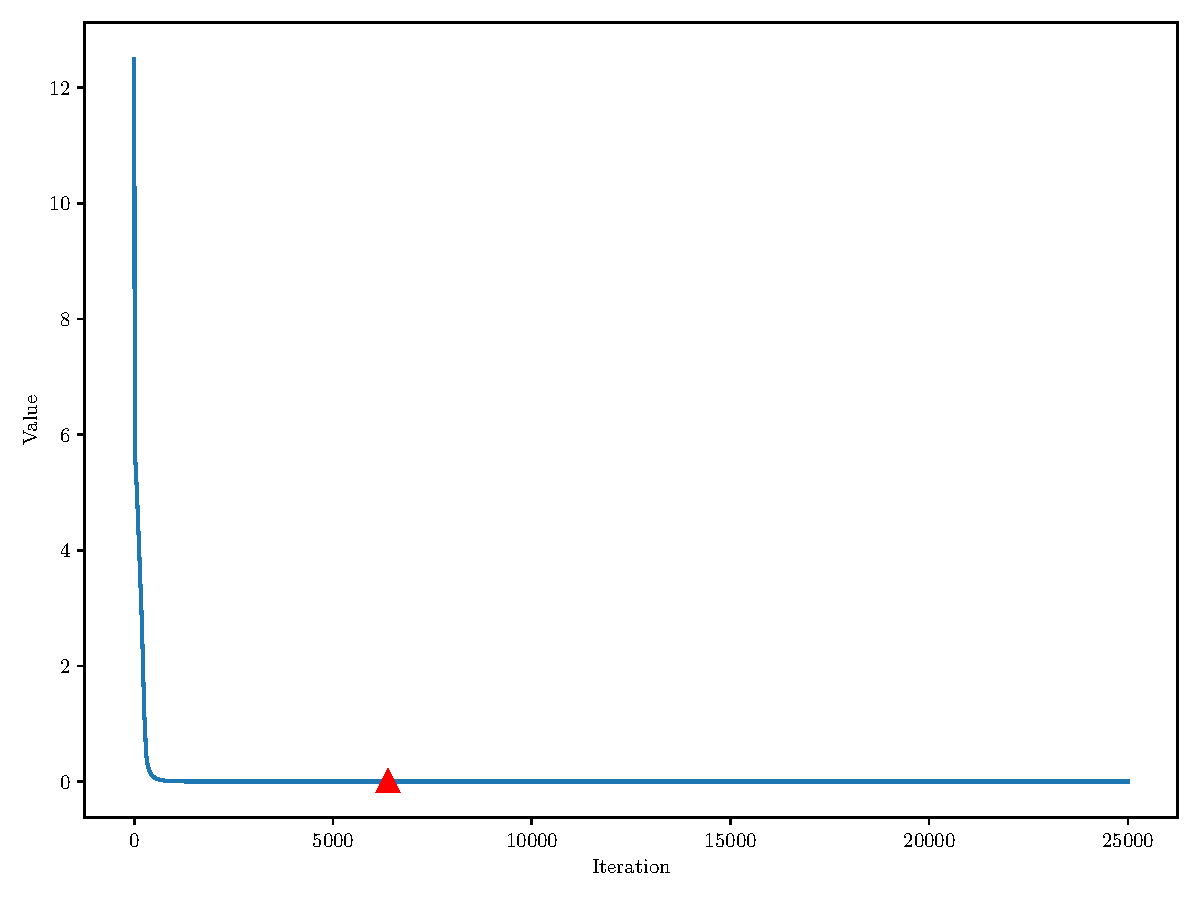
\includegraphics[width=\textwidth]{figures/Krylov_loss.pdf}
        \caption{最优值收敛曲线}
    \end{subfigure}
    \begin{subfigure}{0.4\textwidth}
        \centering
        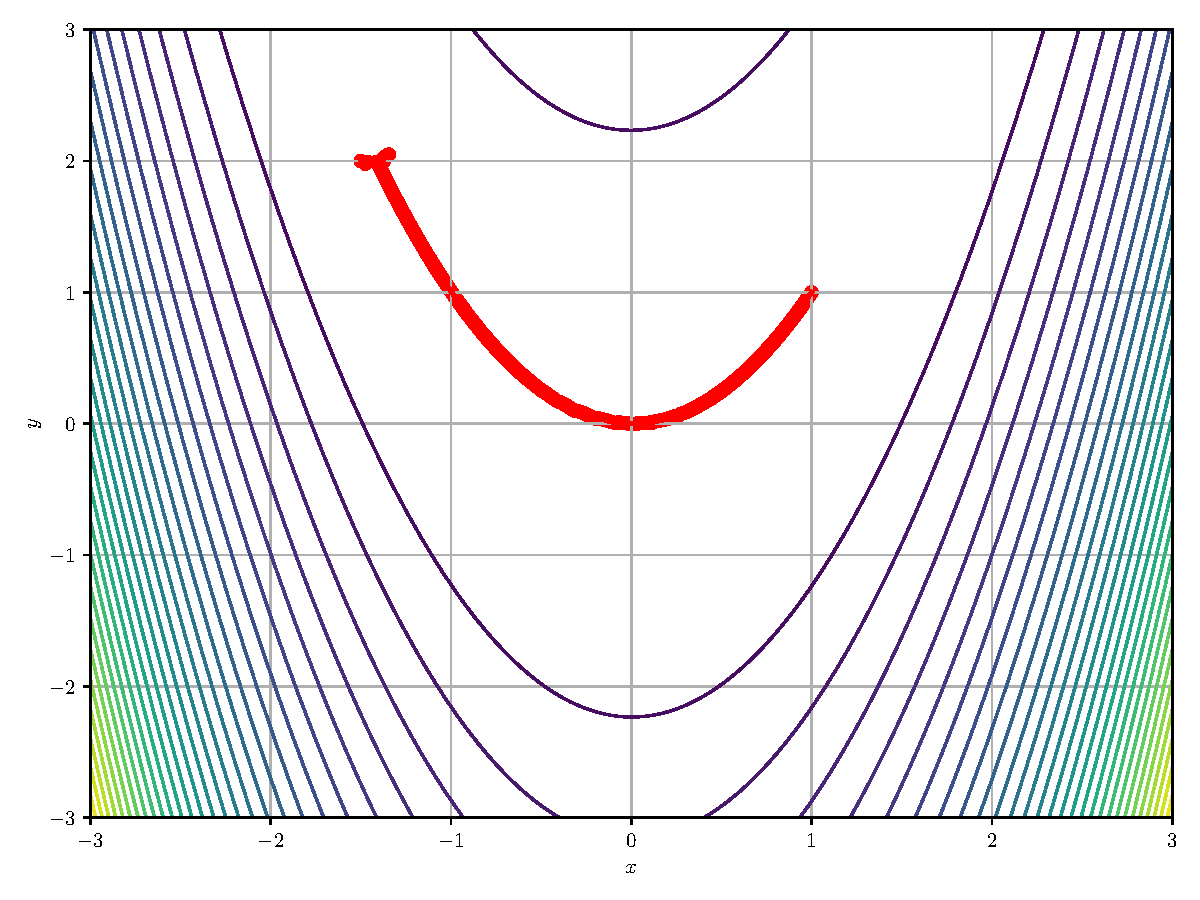
\includegraphics[width=\textwidth]{figures/Krylov_points.pdf}
        \caption{最优点收敛路径}
    \end{subfigure}
    \caption{Krylov的最优值收敛曲线与最优点收敛路径}
    \label{figure:krylov}
\end{figure}

从各图可看出,各优化器均在较少的迭代轮次内下降至最优值附近,但各优化器迭代至最优点需要的迭代轮次总和不同。
综合\cref{table:result}可知,Newton法所需要的迭代轮次最少。

鉴于Random Search优化器对初始随机种子较为敏感,实验对多个随机种子进行了实验比较,结果显示使用种子42时所需迭代轮次较少,因此在实验中固定采用该种子。

从\cref{figure:random search}中可看出,Random Search优化器也在较少的迭代轮次下收敛到最优点。

    \section{结论}

本次实验系统地梳理了多种优化方法的原理与特性,并通过PyTorch框架实现了这些算法。
使用Rosenbrock函数对各法进行了性能评估,从\cref{figure:random search}至\cref{figure:krylov}与\cref{table:result}中可以深入分析各法的表现。

从各法的最优值收敛曲线来看,大部分方法在迭代初期能够迅速降低目标函数值。
然而,具体收敛速度随着时间推移呈现出明显差异。
例如随机搜索法在初期表现较为波动,但随着迭代次数增加,其目标函数值逐渐稳定并接近最优值。
而梯度下降法与次梯度下降法在初期的收敛速度相对缓慢,但随着迭代次数增加,逐渐展现出稳定的下降趋势,最终逼近最优解。

在最优点收敛路径方面,不同法呈现出独特的路径特征。
共轭方向法与共轭梯度法表现出较为直接的收敛路径,能够在较少的迭代步骤中找到最优解附近的位置。
相较于一阶方法,BFGS法通过近似二阶信息,在迭代过程中展现出更快的收敛速度,其路径也更为平滑。

从\cref{table:result}中可以看出,Newton法在所有方法中所需的迭代轮次最少,这得益于其充分利用了二阶导数信息,从而实现对目标函数的二次逼近,展现出极高的收敛效率。
阻尼Newton法虽然在一定程度上增加了计算复杂度,但通过阻尼因子的引入,有效避免了Newton法可能出现的发散问题,同时保持了较快的收敛速度。

在SGD法的表现中,我们可以观察到其在大规模样本问题中的潜力。
虽然在本次实验中使用的是固定的目标函数,但SGD通过对随机样本的更新策略,在迭代过程中依然能够逐步接近最优解,显示出其在处理大规模数据集时的适用性。

ADMM法主要用于分布式优化和带有约束条件的问题。
从实验结果来看,ADMM在处理具有分离结构的优化问题时,能够有效地分解原问题,通过交替更新变量和乘子,最终实现对原问题的求解。
其收敛路径表现出一定的波动性,但在迭代过程中仍能逐步逼近最优解。

从整体的实验结果来看,各法均能够有效地在一定迭代次数内将目标函数值降至接近最优值的水平。
但从收敛速度和迭代轮次的角度分析,Newton法及其改进形式(阻尼Newton法)展现出明显的优势。
然而,这种优势的取得是以计算二阶导数信息为代价的,因此在实际应用中需要权衡计算复杂度和收敛速度之间的关系。

在面对高维大规模问题时,Krylov子空间方法等迭代策略展现出了其独特的优势。
这种基于子空间投影的优化策略,能够在较低的计算成本下逐步逼近最优解,为高维问题的求解提供了有效的途径。
从随机搜索法的表现中,我们也可以得到一些启发。
尽管其收敛速度相对较慢,但在某些特定场景下,例如目标函数难以求导或导数信息不可靠时,随机搜索法作为一种无需梯度信息的优化方法,仍具有其独特的应用价值。

\end{document}
